\documentclass{article}
\usepackage{graphicx} % Required for inserting images
\usepackage{geometry}
\usepackage{circuitikz}
\usepackage{siunitx}
\usepackage{CJKutf8}
\usepackage{amsmath}
\usepackage{amssymb}
\usepackage{caption}
\usepackage{float}
\usepackage{subcaption}
\geometry{top=10mm, left=20mm, a4paper}




\title{Antoniou Inductance-Simulation Circuit Report}
\author{梁程捷 (B11901136), 吳奕娃 (B11901080)}
\date{}


\begin{document}
\begin{CJK*}{UTF8}{bkai}
\maketitle

\section*{Antoniou Inductance-Simulation Circuit}

\begin{figure}[h]
    \begin{center}
        \begin{subfigure}[b]{0.45\textwidth}
            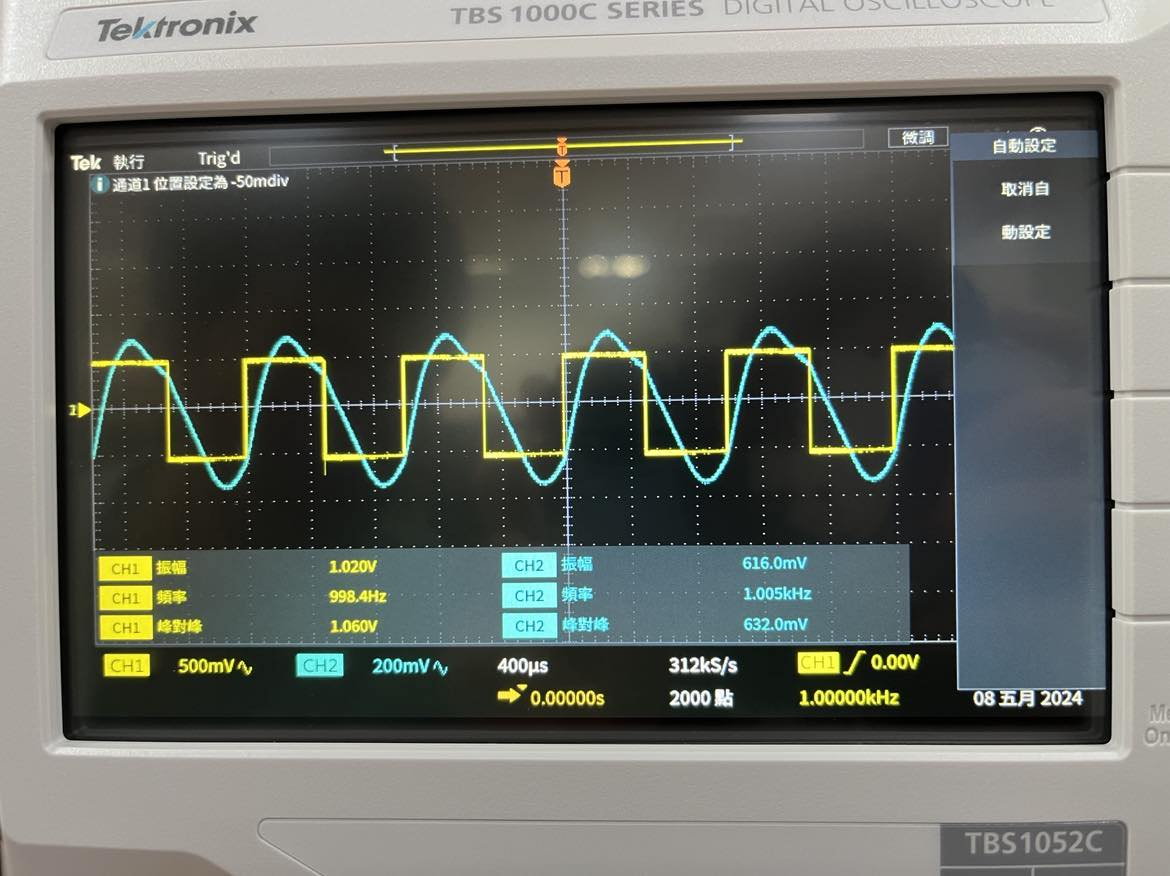
\includegraphics[width=\textwidth]{1st_harmonic.jpg}
            \caption*{Waveforms of $V_o$ for $R_5$ = 10 \unit{\kilo\ohm}.}
        \end{subfigure}
        ~
        \begin{subfigure}[b]{0.45\textwidth}
            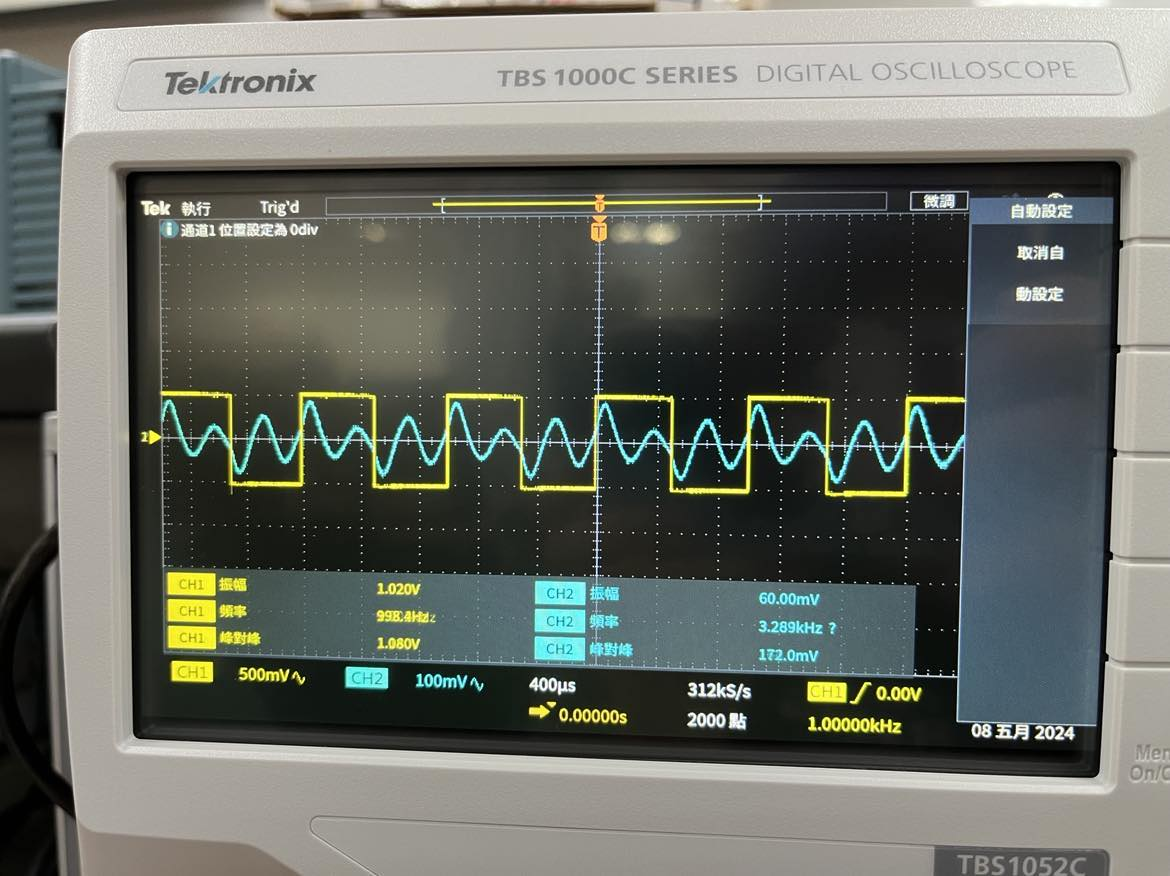
\includegraphics[width=\textwidth]{3rd_harmonic.jpg}
            \caption*{Waveforms of $V_o$ for $R_5$ = 1.1 \unit{\kilo\ohm}.}
        \end{subfigure}
    \end{center}
\end{figure}

\begin{figure}[h]
    \begin{center}
        \begin{subfigure}[b]{0.45\textwidth}
            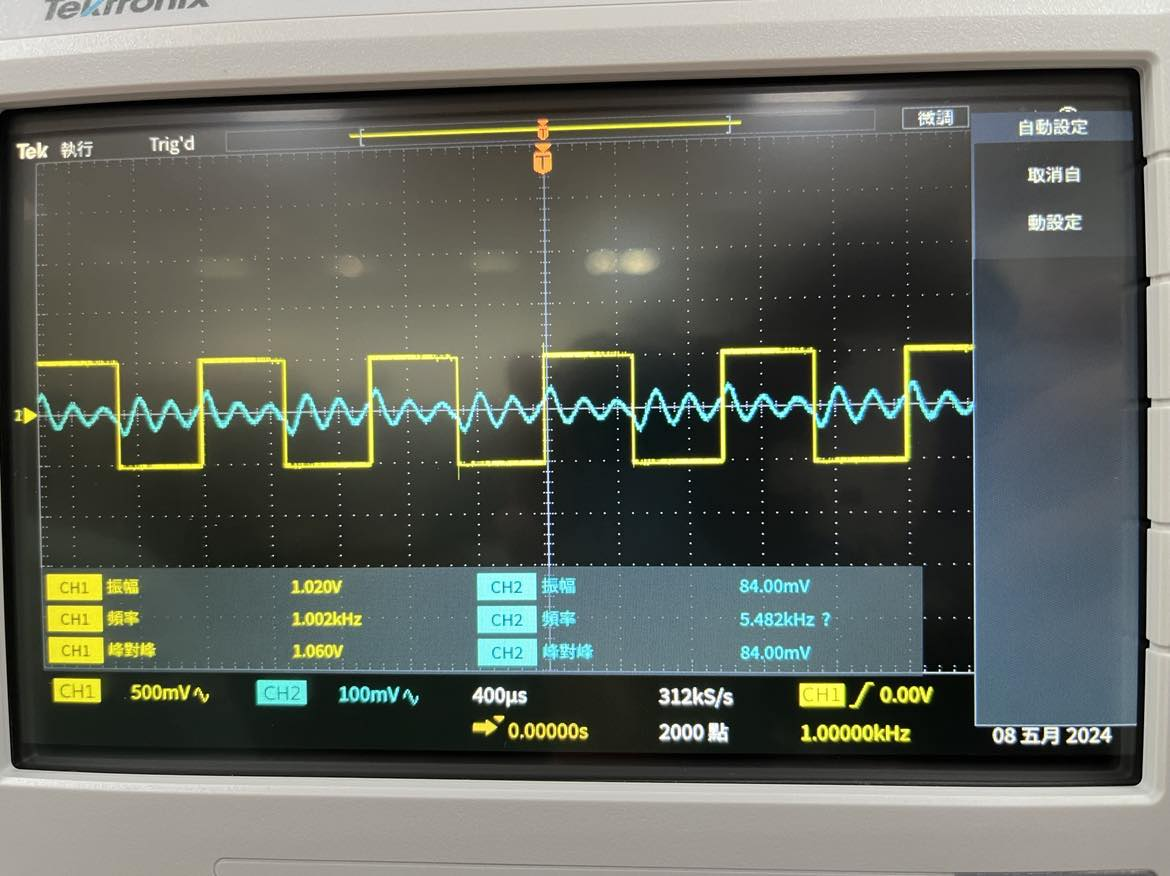
\includegraphics[width=\textwidth]{5th_harmonic.jpg}
            \caption*{Waveforms of $V_o$ for $R_5$ = 400 \unit{\ohm}.}
        \end{subfigure}
        ~
        \begin{subfigure}[b]{0.45\textwidth}
            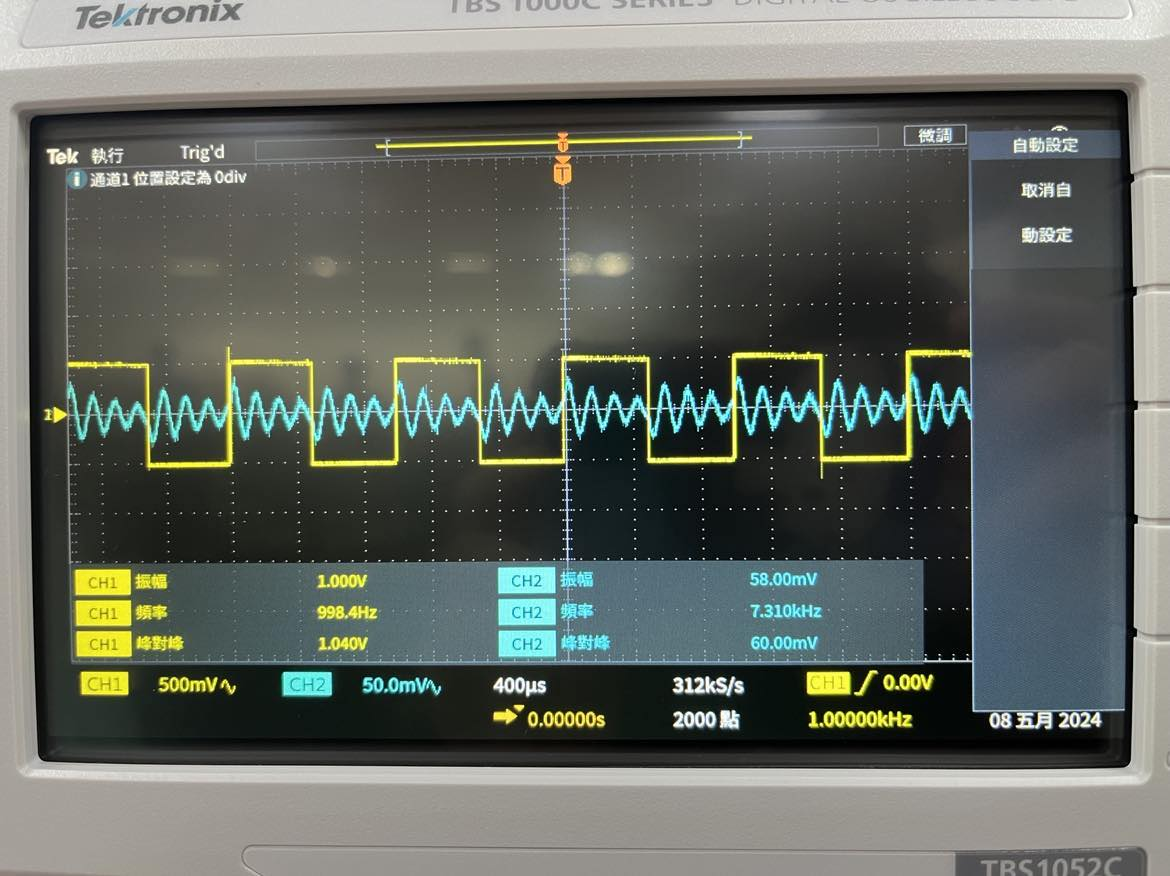
\includegraphics[width=\textwidth]{7th_harmonic.jpg}
            \caption*{Waveforms of $V_o$ for $R_5$ = 200 \unit{\ohm}.}
        \end{subfigure}
    \end{center}
\end{figure}

\section*{Reflections}
\subsection*{梁程捷}
這次實驗的電路很有趣,能實作不用電感,但做出等效電感的效果,并且改變電感值,讓電路在不同的模態下共振。
\subsection*{吳奕娃}
這次的實驗感覺很好玩,調整可變電阻可以看到輸出波型從一次諧波到七次諧波的變化過程,非常有趣。

\end{CJK*}
\end{document}